\begin{figure}[htbp]
\centering
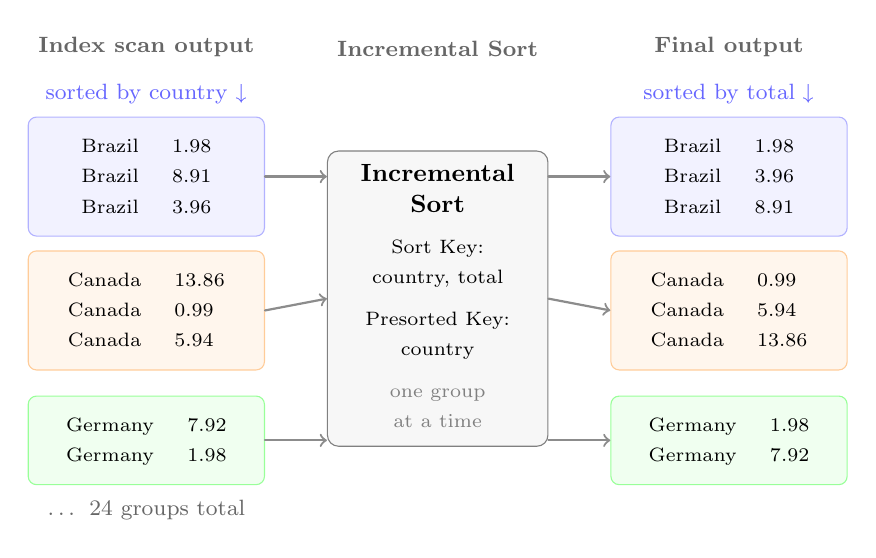
\begin{tikzpicture}[
  font=\small,
  arr/.style={->, black!45, thick, line cap=round},
  box/.style={draw=black!30, fill=black!4, rounded corners=3pt,
              minimum width=2.8cm, minimum height=0.55cm,
              inner xsep=6pt, inner ysep=3pt, align=left},
  grpbox/.style={draw, rounded corners=3pt, inner sep=5pt},
  lbl/.style={font=\footnotesize, black!60},
]

%% ── column headers ────────────────────────────────────────────────
\node[lbl, anchor=south] at (1.8, 4.8)  {\textbf{Index scan output}};
\node[lbl, anchor=south] at (5.5, 4.8)  {\textbf{Incremental Sort}};
\node[lbl, anchor=south] at (9.2, 4.8)  {\textbf{Final output}};

%% ═══ LEFT: index output (pre-sorted on leading key) ══════════════
% Group A — Brazil
\node[grpbox, fill=blue!5,  draw=blue!30,  minimum width=3cm] (GA)
  at (1.8, 3.4)
  {\begin{tabular}{ll}
     \scriptsize Brazil & \scriptsize 1.98 \\
     \scriptsize Brazil & \scriptsize 8.91 \\
     \scriptsize Brazil & \scriptsize 3.96 \\
   \end{tabular}};
\node[lbl, above=1pt] at (GA.north) {\footnotesize\color{blue!60}sorted by country ↓};

% Group B — Canada
\node[grpbox, fill=orange!7, draw=orange!40, minimum width=3cm] (GB)
  at (1.8, 1.7)
  {\begin{tabular}{ll}
     \scriptsize Canada & \scriptsize 13.86 \\
     \scriptsize Canada & \scriptsize 0.99  \\
     \scriptsize Canada & \scriptsize 5.94  \\
   \end{tabular}};

% Group C — Germany
\node[grpbox, fill=green!6, draw=green!40, minimum width=3cm] (GC)
  at (1.8, 0.05)
  {\begin{tabular}{ll}
     \scriptsize Germany & \scriptsize 7.92  \\
     \scriptsize Germany & \scriptsize 1.98  \\
   \end{tabular}};

\node[lbl, below=2pt] at (GC.south) {\footnotesize … 24 groups total};

%% ═══ MIDDLE: Incremental Sort node ══════════════════════════════
\node[draw=black!50, fill=gray!6, rounded corners=4pt,
      minimum width=2.8cm, minimum height=3.6cm, align=center] (IS)
  at (5.5, 1.85)
  {\begin{tabular}{c}
     \textbf{Incremental}\\
     \textbf{Sort}\\[4pt]
     \scriptsize Sort Key:\\
     \scriptsize country, total\\[4pt]
     \scriptsize Presorted Key:\\
     \scriptsize country\\[4pt]
     \scriptsize\color{black!50}one group\\
     \scriptsize\color{black!50}at a time
   \end{tabular}};

%% arrows left → middle
\draw[arr] (GA.east) -- (IS.north west |- GA.east);
\draw[arr] (GB.east) -- (IS.west);
\draw[arr] (GC.east) -- (IS.south west |- GC.east);

%% ═══ RIGHT: sorted output per group ══════════════════════════════
% Group A sorted
\node[grpbox, fill=blue!5, draw=blue!30, minimum width=3cm] (RA)
  at (9.2, 3.4)
  {\begin{tabular}{ll}
     \scriptsize Brazil & \scriptsize 1.98 \\
     \scriptsize Brazil & \scriptsize 3.96 \\
     \scriptsize Brazil & \scriptsize 8.91 \\
   \end{tabular}};
\node[lbl, above=1pt] at (RA.north) {\footnotesize\color{blue!60}sorted by total ↓};

% Group B sorted
\node[grpbox, fill=orange!7, draw=orange!40, minimum width=3cm] (RB)
  at (9.2, 1.7)
  {\begin{tabular}{ll}
     \scriptsize Canada & \scriptsize 0.99  \\
     \scriptsize Canada & \scriptsize 5.94  \\
     \scriptsize Canada & \scriptsize 13.86 \\
   \end{tabular}};

% Group C sorted
\node[grpbox, fill=green!6, draw=green!40, minimum width=3cm] (RC)
  at (9.2, 0.05)
  {\begin{tabular}{ll}
     \scriptsize Germany & \scriptsize 1.98 \\
     \scriptsize Germany & \scriptsize 7.92 \\
   \end{tabular}};

%% arrows middle → right
\draw[arr] (IS.north east |- RA.west) -- (RA.west);
\draw[arr] (IS.east)                  -- (RB.west);
\draw[arr] (IS.south east |- RC.west) -- (RC.west);

\end{tikzpicture}
\caption{Incremental sort: per-group bounded sort on a partially pre-ordered stream.}
\label{fig:incrementalsort}
\end{figure}
